\section{Experiments}\label{sec:exp}

%\begin{figure}[!h]
%\centering
%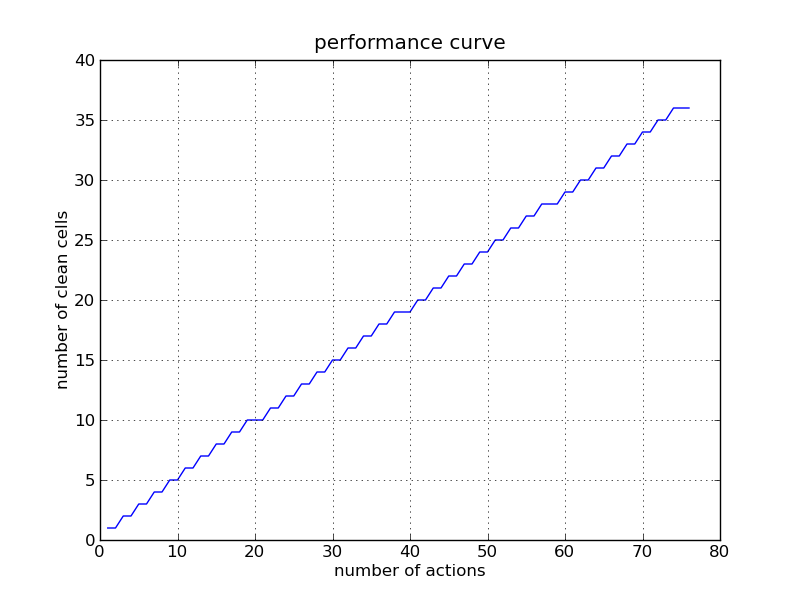
\includegraphics[scale=.35]{img/agent1.png}
%\caption{Performance of Memoryless Deterministic Agent}
%\label{fig:agent1}
%\end{figure}

%\begin{table}[h]
%    \centering
%    \begin{tabular}{|l|c|c|c|c|c|c|c|c|c|c|}
%        \hline
%        trials 1-10 & 495 & 625 & 514 & 647 & 842 & 614 & 550 & 532 & 532 & 924\\ \hline
%        trials 11-20 & 510 & 585 & 519 & 616 & 504 & 434 & 477 & 538 & 489 & 479\\ \hline
%        trials 21-30 & 385 & 562 & 531 & 591 & 551 & 458 & 515 & 711 & 662 & 439\\ \hline
%        trials 31-40 & 461 & 398 & 604 & 601 & 900 & 428 & 507 & 594 & 512 & 735\\ \hline
%        trials 41-50 & 572 & 574 & 490 & 498 & 578 & 517 & 380 & 444 & 605 & 506\\ \hline
%    \end{tabular}
%    \caption{Number of actions to take to clean $90\%$ of the room}\label{tab:agent2}
%\end{table}

%\begin{figure}[!h]
%        \centering
%        \subfloat[Number of actions]{
%                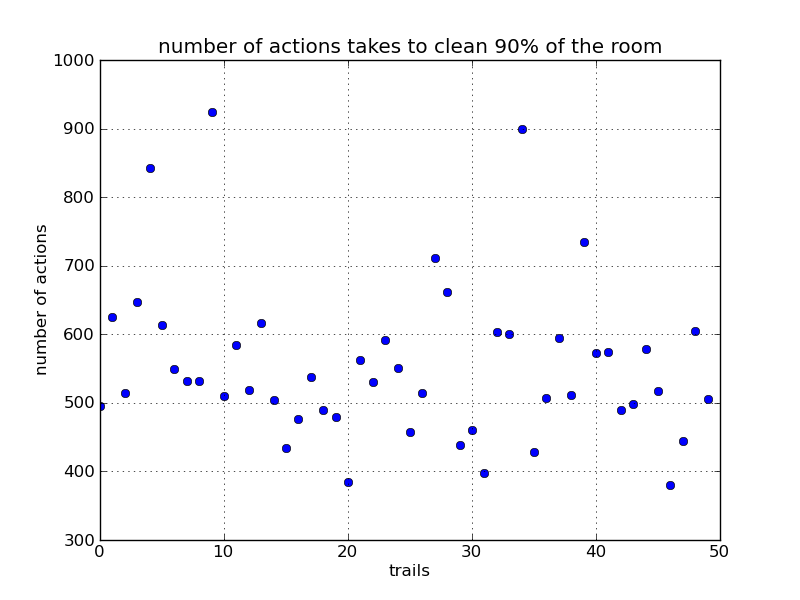
\includegraphics[scale=0.35]{img/num_actions.png}
%        }
%        \hspace{0.5in}
%        \subfloat[Performance curves]{
%                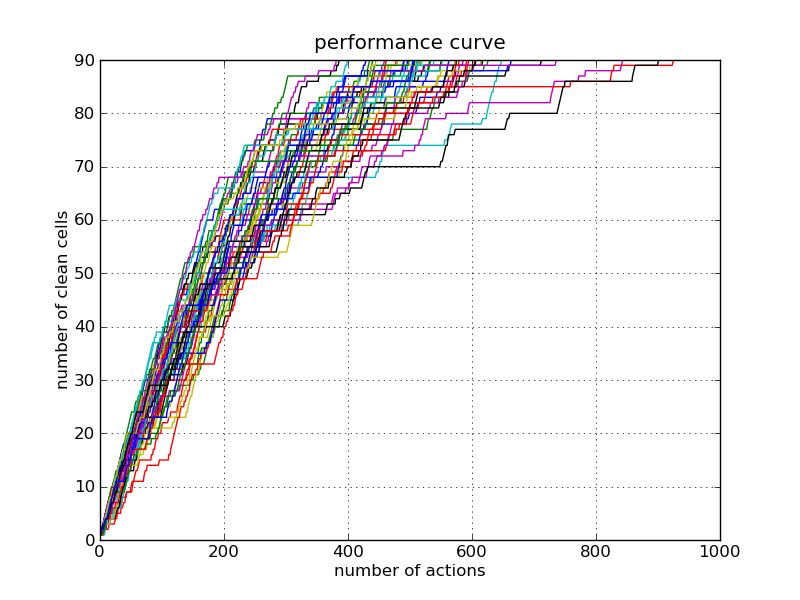
\includegraphics[scale=0.35]{img/rand.png}
%        }
%        \caption{Performance of randomized reflex agent}\label{fig:agent2}
%\end{figure}

\subsection{Heuristics}
We observed that the length of a path is the steps moving from initial state to goal state. So a natural heuristic can be designed based on an optimistic estimation of how many steps need to turn a state to its final goal. The first admissible heuristic is as following:
\[
h(s) = (\sum_i |pegs(1,i)-i| ) + numberDisks(pegs(2)) + numberDisks(pegs(3))
\]
The intuition is for a disk $k$ in peg $1$, it has to take $|k-i|$ steps to get to the place it should be, where $i$ is its current location on the peg. For example, if the $9th$ disk on the bottom, it has to take $9-0$ steps to get to the top. For disks on peg $2$ and peg $3$, they have to be moved from current location to peg $1$ in at least $1$ step. This is in fact an admissible heuristic. We are not going to prove it here. A simple justification is given as follow. For any disk on peg $1$, before it reaches to its ideal position, there should be $|k-i|$ disks put underneath it, and for every such disk, takes at least $1$ step. 

\subsection{Results}

\begin{table}[h]
    \centering
    \begin{tabular}{|l|c|c|c|c|c|c|c}
        \hline
        Disks: & 4 & 5 & 6 & 7 & 8 & 9 & 10\\ \hline
        A*/admissible & 8.85 & 11.85 & 14.6 & 17.5 & 20.2 & 24.1 & 27.6\\ \hline
        A*/nonadmissible & 8.85 & 11.85 & 15.25 & 19 & 22.21 & 26.81 & 32.25 \\ \hline
        RBFS/admissible & 9.25 & 12.95 & 16.5 & 20.05 & 23.8 & 27.4 & 34.05\\ \hline
        RBFS/nonadmissible & 11.25 & 17.85 & 24.35 & 32.75 & 40.35 & 50.7 & 64.55\\ \hline
    \end{tabular}
    \caption{Average solution length per algorithm, heuristic and disk size.}\label{tab:solen}
\end{table}


